\documentclass[]{article}
\usepackage{lmodern}
\usepackage{amssymb,amsmath}
\usepackage{ifxetex,ifluatex}
\usepackage{fixltx2e} % provides \textsubscript
\ifnum 0\ifxetex 1\fi\ifluatex 1\fi=0 % if pdftex
  \usepackage[T1]{fontenc}
  \usepackage[utf8]{inputenc}
\else % if luatex or xelatex
  \ifxetex
    \usepackage{mathspec}
  \else
    \usepackage{fontspec}
  \fi
  \defaultfontfeatures{Ligatures=TeX,Scale=MatchLowercase}
\fi
% use upquote if available, for straight quotes in verbatim environments
\IfFileExists{upquote.sty}{\usepackage{upquote}}{}
% use microtype if available
\IfFileExists{microtype.sty}{%
\usepackage{microtype}
\UseMicrotypeSet[protrusion]{basicmath} % disable protrusion for tt fonts
}{}
\usepackage[margin=1in]{geometry}
\usepackage{hyperref}
\hypersetup{unicode=true,
            pdftitle={随机模拟方法与应用导论 作业七},
            pdfauthor={陈稼霖 45875852},
            pdfborder={0 0 0},
            breaklinks=true}
\urlstyle{same}  % don't use monospace font for urls
\usepackage{color}
\usepackage{fancyvrb}
\newcommand{\VerbBar}{|}
\newcommand{\VERB}{\Verb[commandchars=\\\{\}]}
\DefineVerbatimEnvironment{Highlighting}{Verbatim}{commandchars=\\\{\}}
% Add ',fontsize=\small' for more characters per line
\usepackage{framed}
\definecolor{shadecolor}{RGB}{248,248,248}
\newenvironment{Shaded}{\begin{snugshade}}{\end{snugshade}}
\newcommand{\AlertTok}[1]{\textcolor[rgb]{0.94,0.16,0.16}{#1}}
\newcommand{\AnnotationTok}[1]{\textcolor[rgb]{0.56,0.35,0.01}{\textbf{\textit{#1}}}}
\newcommand{\AttributeTok}[1]{\textcolor[rgb]{0.77,0.63,0.00}{#1}}
\newcommand{\BaseNTok}[1]{\textcolor[rgb]{0.00,0.00,0.81}{#1}}
\newcommand{\BuiltInTok}[1]{#1}
\newcommand{\CharTok}[1]{\textcolor[rgb]{0.31,0.60,0.02}{#1}}
\newcommand{\CommentTok}[1]{\textcolor[rgb]{0.56,0.35,0.01}{\textit{#1}}}
\newcommand{\CommentVarTok}[1]{\textcolor[rgb]{0.56,0.35,0.01}{\textbf{\textit{#1}}}}
\newcommand{\ConstantTok}[1]{\textcolor[rgb]{0.00,0.00,0.00}{#1}}
\newcommand{\ControlFlowTok}[1]{\textcolor[rgb]{0.13,0.29,0.53}{\textbf{#1}}}
\newcommand{\DataTypeTok}[1]{\textcolor[rgb]{0.13,0.29,0.53}{#1}}
\newcommand{\DecValTok}[1]{\textcolor[rgb]{0.00,0.00,0.81}{#1}}
\newcommand{\DocumentationTok}[1]{\textcolor[rgb]{0.56,0.35,0.01}{\textbf{\textit{#1}}}}
\newcommand{\ErrorTok}[1]{\textcolor[rgb]{0.64,0.00,0.00}{\textbf{#1}}}
\newcommand{\ExtensionTok}[1]{#1}
\newcommand{\FloatTok}[1]{\textcolor[rgb]{0.00,0.00,0.81}{#1}}
\newcommand{\FunctionTok}[1]{\textcolor[rgb]{0.00,0.00,0.00}{#1}}
\newcommand{\ImportTok}[1]{#1}
\newcommand{\InformationTok}[1]{\textcolor[rgb]{0.56,0.35,0.01}{\textbf{\textit{#1}}}}
\newcommand{\KeywordTok}[1]{\textcolor[rgb]{0.13,0.29,0.53}{\textbf{#1}}}
\newcommand{\NormalTok}[1]{#1}
\newcommand{\OperatorTok}[1]{\textcolor[rgb]{0.81,0.36,0.00}{\textbf{#1}}}
\newcommand{\OtherTok}[1]{\textcolor[rgb]{0.56,0.35,0.01}{#1}}
\newcommand{\PreprocessorTok}[1]{\textcolor[rgb]{0.56,0.35,0.01}{\textit{#1}}}
\newcommand{\RegionMarkerTok}[1]{#1}
\newcommand{\SpecialCharTok}[1]{\textcolor[rgb]{0.00,0.00,0.00}{#1}}
\newcommand{\SpecialStringTok}[1]{\textcolor[rgb]{0.31,0.60,0.02}{#1}}
\newcommand{\StringTok}[1]{\textcolor[rgb]{0.31,0.60,0.02}{#1}}
\newcommand{\VariableTok}[1]{\textcolor[rgb]{0.00,0.00,0.00}{#1}}
\newcommand{\VerbatimStringTok}[1]{\textcolor[rgb]{0.31,0.60,0.02}{#1}}
\newcommand{\WarningTok}[1]{\textcolor[rgb]{0.56,0.35,0.01}{\textbf{\textit{#1}}}}
\usepackage{graphicx,grffile}
\makeatletter
\def\maxwidth{\ifdim\Gin@nat@width>\linewidth\linewidth\else\Gin@nat@width\fi}
\def\maxheight{\ifdim\Gin@nat@height>\textheight\textheight\else\Gin@nat@height\fi}
\makeatother
% Scale images if necessary, so that they will not overflow the page
% margins by default, and it is still possible to overwrite the defaults
% using explicit options in \includegraphics[width, height, ...]{}
\setkeys{Gin}{width=\maxwidth,height=\maxheight,keepaspectratio}
\IfFileExists{parskip.sty}{%
\usepackage{parskip}
}{% else
\setlength{\parindent}{0pt}
\setlength{\parskip}{6pt plus 2pt minus 1pt}
}
\setlength{\emergencystretch}{3em}  % prevent overfull lines
\providecommand{\tightlist}{%
  \setlength{\itemsep}{0pt}\setlength{\parskip}{0pt}}
\setcounter{secnumdepth}{0}
% Redefines (sub)paragraphs to behave more like sections
\ifx\paragraph\undefined\else
\let\oldparagraph\paragraph
\renewcommand{\paragraph}[1]{\oldparagraph{#1}\mbox{}}
\fi
\ifx\subparagraph\undefined\else
\let\oldsubparagraph\subparagraph
\renewcommand{\subparagraph}[1]{\oldsubparagraph{#1}\mbox{}}
\fi

%%% Use protect on footnotes to avoid problems with footnotes in titles
\let\rmarkdownfootnote\footnote%
\def\footnote{\protect\rmarkdownfootnote}

%%% Change title format to be more compact
\usepackage{titling}

% Create subtitle command for use in maketitle
\providecommand{\subtitle}[1]{
  \posttitle{
    \begin{center}\large#1\end{center}
    }
}

\setlength{\droptitle}{-2em}

  \title{随机模拟方法与应用导论 作业七}
    \pretitle{\vspace{\droptitle}\centering\huge}
  \posttitle{\par}
    \author{陈稼霖 45875852}
    \preauthor{\centering\large\emph}
  \postauthor{\par}
      \predate{\centering\large\emph}
  \postdate{\par}
    \date{2019-10-05}

\usepackage[UTF8]{ctex}

\begin{document}
\maketitle

\hypertarget{hubbles-law}{%
\section{7.5 (Hubble's Law)}\label{hubbles-law}}

In 1929 Edwin Hubble investigated the relationship between distance and
velocity of celestial objects. Knowledge of this relationship might give
clues as to how the universe was formed and what may happen in the
future. Hubble's Law is \[
\text{Recession Velocity}=H_0\times\text{Distance}
\] where \(H_0\) is Hubble's constant. This model is a straight line
through the origin with slope \(H_0\). Data that Hubble used to estimate
the constant \(H_0\) are given on the DASL web at
\url{http://lib.stat.cmu.edu/DASL/Datafiles/Hubble.html}. Use the data
to estimate Hubble's constant by simple linear regression.

首先读取储存有数据的文件\texttt{hubble.xls},数据如下

\begin{Shaded}
\begin{Highlighting}[]
\NormalTok{hubble =}\StringTok{ }\KeywordTok{read.table}\NormalTok{(}\StringTok{'hubble.txt'}\NormalTok{,}\DataTypeTok{header =} \OtherTok{TRUE}\NormalTok{)}
\NormalTok{hubble}
\end{Highlighting}
\end{Shaded}

\begin{verbatim}
##    distance recession_velocity
## 1     0.032                170
## 2     0.034                290
## 3     0.214               -130
## 4     0.263                -70
## 5     0.275               -185
## 6     0.275               -220
## 7     0.450                200
## 8     0.500                290
## 9     0.500                270
## 10    0.630                200
## 11    0.800                300
## 12    0.900                -30
## 13    0.900                650
## 14    0.900                150
## 15    0.900                500
## 16    1.000                920
## 17    1.100                450
## 18    1.100                500
## 19    1.400                500
## 20    1.700                960
## 21    2.000                500
## 22    2.000                850
## 23    2.000                800
## 24    2.000               1090
\end{verbatim}

然后调用函数\texttt{lm},用过原点的一条直线拟合上面的数据,展示拟合直线的斜率和图像

\begin{Shaded}
\begin{Highlighting}[]
\NormalTok{M1 =}\StringTok{ }\KeywordTok{lm}\NormalTok{(hubble}\OperatorTok{$}\NormalTok{recession_velocity }\OperatorTok{~}\StringTok{ }\DecValTok{0} \OperatorTok{+}\StringTok{ }\NormalTok{hubble}\OperatorTok{$}\NormalTok{distance)}
\NormalTok{M1}
\end{Highlighting}
\end{Shaded}

\begin{verbatim}
## 
## Call:
## lm(formula = hubble$recession_velocity ~ 0 + hubble$distance)
## 
## Coefficients:
## hubble$distance  
##           423.9
\end{verbatim}

\begin{Shaded}
\begin{Highlighting}[]
\KeywordTok{plot}\NormalTok{(hubble,}\DataTypeTok{main =} \StringTok{'The Relationship Between Distance and Velocity of Celestial Objects'}\NormalTok{)}
\KeywordTok{abline}\NormalTok{(M1)}
\end{Highlighting}
\end{Shaded}

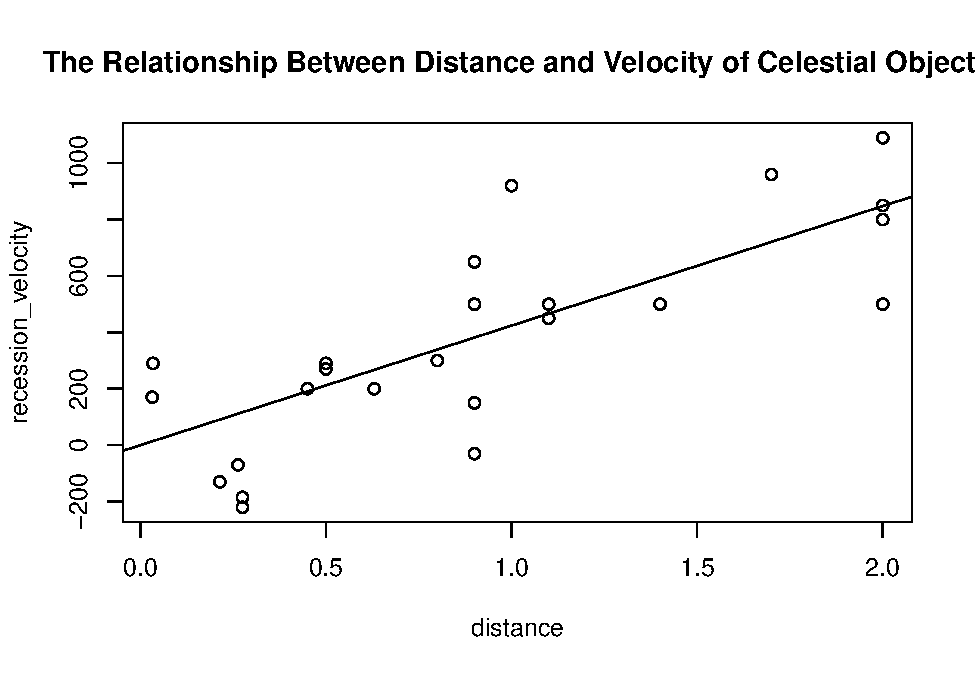
\includegraphics{Homework_7_files/figure-latex/unnamed-chunk-2-1.pdf}

由此可见,哈勃常数(拟合直线的斜率)\(H_0=432.9\) \[
\text{Recession Velocity}=432.9\times\text{Distance}
\] 这意味着天体距离每增加\(1\)Mpc,其推行速度增加\(432.9\)km/s。

\hypertarget{lunatics-data}{%
\section{7.10 (lunatics data)}\label{lunatics-data}}

Refer to the ``lunatics'' data in Example 7.8. Repeat the analysis,
after deleting the two counties that are offshore islands,
\texttt{NANTUCKET} and \texttt{DUCKS} counties. Compare the estimates of
slope and intercept with those obtained in Example 7.8. Construct the
plots and analyze the residuals as in Example 7.8.

首选读取储存有数据的文件\texttt{lunatics.txt},数据如下

\begin{Shaded}
\begin{Highlighting}[]
\NormalTok{lunatics =}\StringTok{ }\KeywordTok{read.table}\NormalTok{(}\StringTok{'lunatics.txt'}\NormalTok{,}\DataTypeTok{header =} \OtherTok{TRUE}\NormalTok{)}
\NormalTok{lunatics}
\end{Highlighting}
\end{Shaded}

\begin{verbatim}
##        COUNTY NBR DIST     POP PDEN PHOME
## 1   BERKSHIRE 119   97  26.656   56    77
## 2    FRANKLIN  84   62  22.260   45    81
## 3   HAMPSHIRE  94   54  23.312   72    75
## 4     HAMPDEN 105   52  18.900   94    69
## 5   WORCESTER 351   20  82.836   98    64
## 6   MIDDLESEX 357   14  66.759  231    47
## 7       ESSEX 377   10  95.004 3252    47
## 8     SUFFOLK 458    4 123.202 3042     6
## 9     NORFOLK 241   14  62.901  235    49
## 10    BRISTOL 158   14  29.704  151    60
## 11   PLYMOUTH 139   16  32.526   91    68
## 12 BARNSTABLE  78   44  16.692   93    76
## 13  NANTUCKET  12   77   1.740  179    25
## 14      DUKES  19   52   7.524   46    79
\end{verbatim}

去除\texttt{COUNTY}为\texttt{NANTUCKET}和\texttt{DUKES}的行

\begin{Shaded}
\begin{Highlighting}[]
\NormalTok{lunatics =}\StringTok{ }\NormalTok{lunatics[}\KeywordTok{which}\NormalTok{(lunatics}\OperatorTok{$}\NormalTok{COUNTY }\OperatorTok{!=}\StringTok{ 'NANTUCKET'} \OperatorTok{&}\StringTok{ }\NormalTok{lunatics}\OperatorTok{$}\NormalTok{COUNTY }\OperatorTok{!=}\StringTok{ 'DUKES'}\NormalTok{),]}
\NormalTok{lunatics}
\end{Highlighting}
\end{Shaded}

\begin{verbatim}
##        COUNTY NBR DIST     POP PDEN PHOME
## 1   BERKSHIRE 119   97  26.656   56    77
## 2    FRANKLIN  84   62  22.260   45    81
## 3   HAMPSHIRE  94   54  23.312   72    75
## 4     HAMPDEN 105   52  18.900   94    69
## 5   WORCESTER 351   20  82.836   98    64
## 6   MIDDLESEX 357   14  66.759  231    47
## 7       ESSEX 377   10  95.004 3252    47
## 8     SUFFOLK 458    4 123.202 3042     6
## 9     NORFOLK 241   14  62.901  235    49
## 10    BRISTOL 158   14  29.704  151    60
## 11   PLYMOUTH 139   16  32.526   91    68
## 12 BARNSTABLE  78   44  16.692   93    76
\end{verbatim}

重复例7.8的分析过程,首先绘制在家照料的疯人百分比\texttt{PHOME}到最近的精神卫生中心的距离\texttt{DIST}的散点图并计算两者的相关系数

\begin{Shaded}
\begin{Highlighting}[]
\KeywordTok{attach}\NormalTok{(lunatics)}
\KeywordTok{plot}\NormalTok{(DIST,PHOME)}
\end{Highlighting}
\end{Shaded}

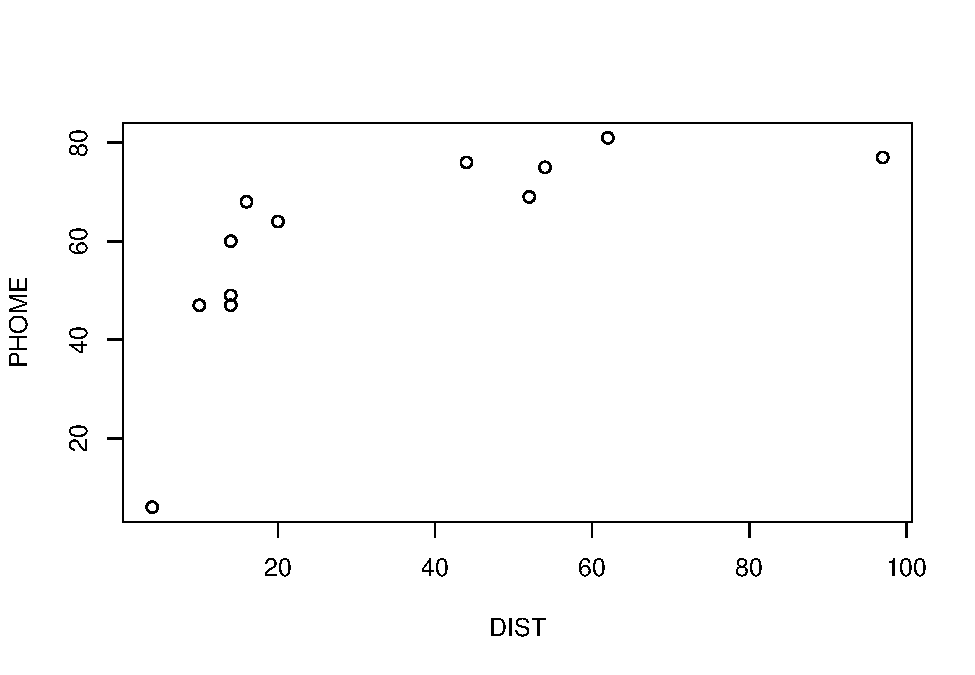
\includegraphics{Homework_7_files/figure-latex/unnamed-chunk-5-1.pdf}

\begin{Shaded}
\begin{Highlighting}[]
\KeywordTok{cor}\NormalTok{(DIST,PHOME)}
\end{Highlighting}
\end{Shaded}

\begin{verbatim}
## [1] 0.6963078
\end{verbatim}

由此可见,\texttt{PHOME}和\texttt{DIST}之间的关系似乎并非线性,而更可能是双曲线。因此,取\texttt{DIST}的倒数\texttt{RDIST},绘制\texttt{PHOME}关于\texttt{RDIST}的散点图,并计算两者之间的相关系数。

\begin{Shaded}
\begin{Highlighting}[]
\NormalTok{RDIST =}\StringTok{ }\DecValTok{1} \OperatorTok{/}\StringTok{ }\NormalTok{DIST}
\KeywordTok{plot}\NormalTok{(RDIST,PHOME)}
\end{Highlighting}
\end{Shaded}

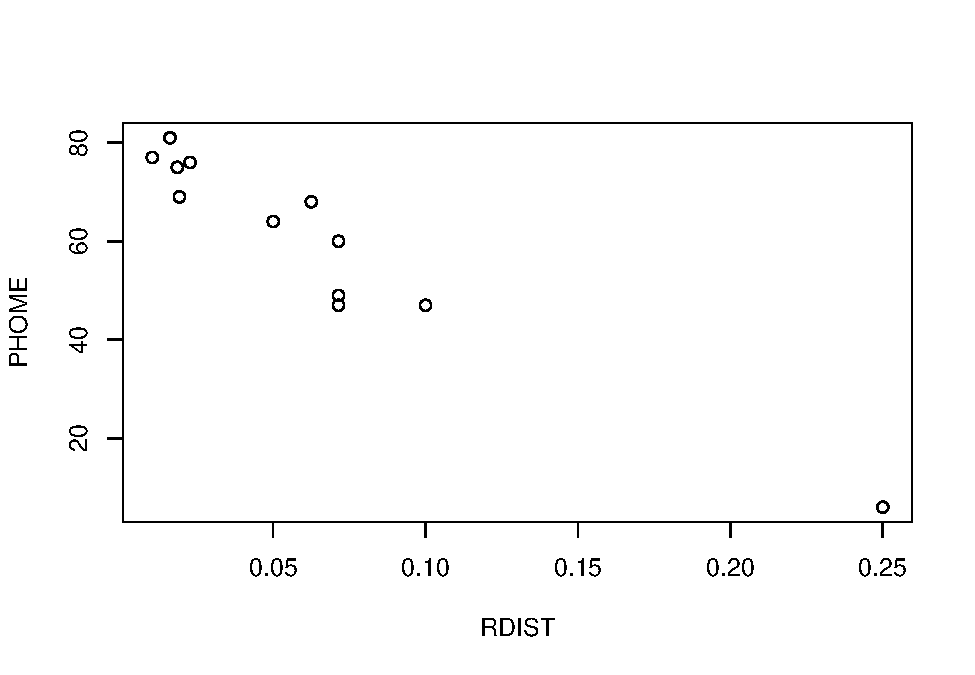
\includegraphics{Homework_7_files/figure-latex/unnamed-chunk-6-1.pdf}

\begin{Shaded}
\begin{Highlighting}[]
\KeywordTok{cor}\NormalTok{(RDIST,PHOME)}
\end{Highlighting}
\end{Shaded}

\begin{verbatim}
## [1] -0.963456
\end{verbatim}

在这里\(|\text{cor(RDIST,PHOME)}|>|\text{cor(DIST,PHOME)}|\),说明\texttt{PHOME}和\texttt{RDIST}之间相对于\texttt{PHOME}和\texttt{RDIST}之间具有更强的线性相关性。因此,我们用简单的线性回归模型
\[
\text{PHOME}_i=\beta_0+\beta_1\text{RDIST}_i+\varepsilon_i
\]
来拟合两者之间的关系,调用函数\texttt{lm}计算相关的参数并绘制相应的拟合线

\begin{Shaded}
\begin{Highlighting}[]
\NormalTok{M2 =}\StringTok{ }\KeywordTok{lm}\NormalTok{(PHOME }\OperatorTok{~}\StringTok{ }\NormalTok{RDIST)}
\NormalTok{M2}
\end{Highlighting}
\end{Shaded}

\begin{verbatim}
## 
## Call:
## lm(formula = PHOME ~ RDIST)
## 
## Coefficients:
## (Intercept)        RDIST  
##       79.36      -305.52
\end{verbatim}

\begin{Shaded}
\begin{Highlighting}[]
\KeywordTok{plot}\NormalTok{(RDIST,PHOME)}
\KeywordTok{abline}\NormalTok{(M2)}
\end{Highlighting}
\end{Shaded}

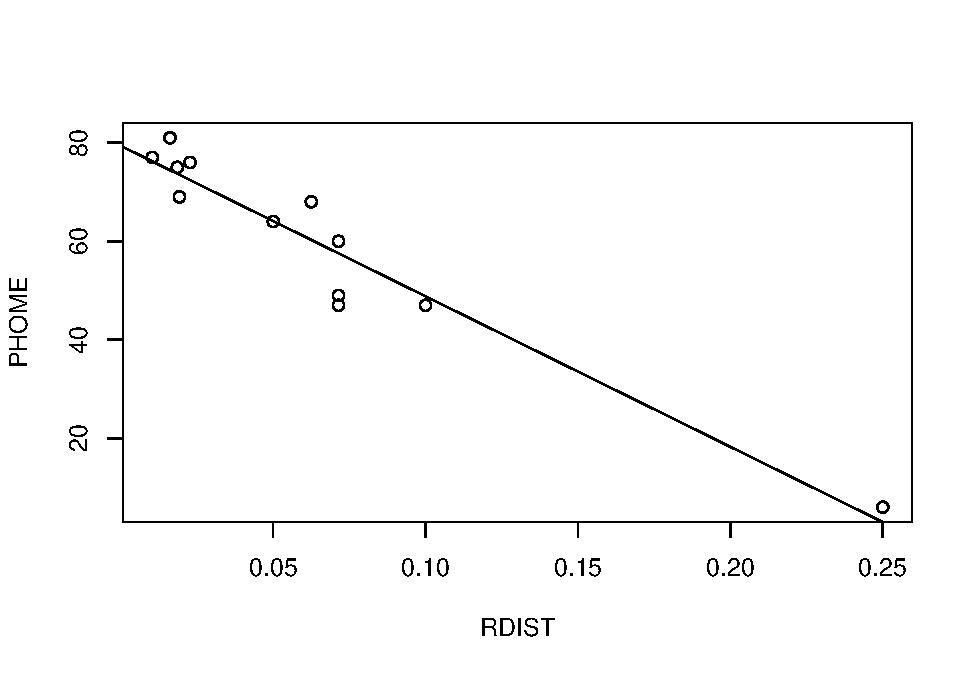
\includegraphics{Homework_7_files/figure-latex/unnamed-chunk-7-1.pdf}

\begin{Shaded}
\begin{Highlighting}[]
\KeywordTok{plot}\NormalTok{(DIST,PHOME)}
\KeywordTok{curve}\NormalTok{(M2}\OperatorTok{$}\NormalTok{coef[}\DecValTok{1}\NormalTok{] }\OperatorTok{+}\StringTok{ }\NormalTok{M2}\OperatorTok{$}\NormalTok{coef[}\DecValTok{2}\NormalTok{] }\OperatorTok{/}\StringTok{ }\NormalTok{x,}\DataTypeTok{add =} \OtherTok{TRUE}\NormalTok{)}
\end{Highlighting}
\end{Shaded}

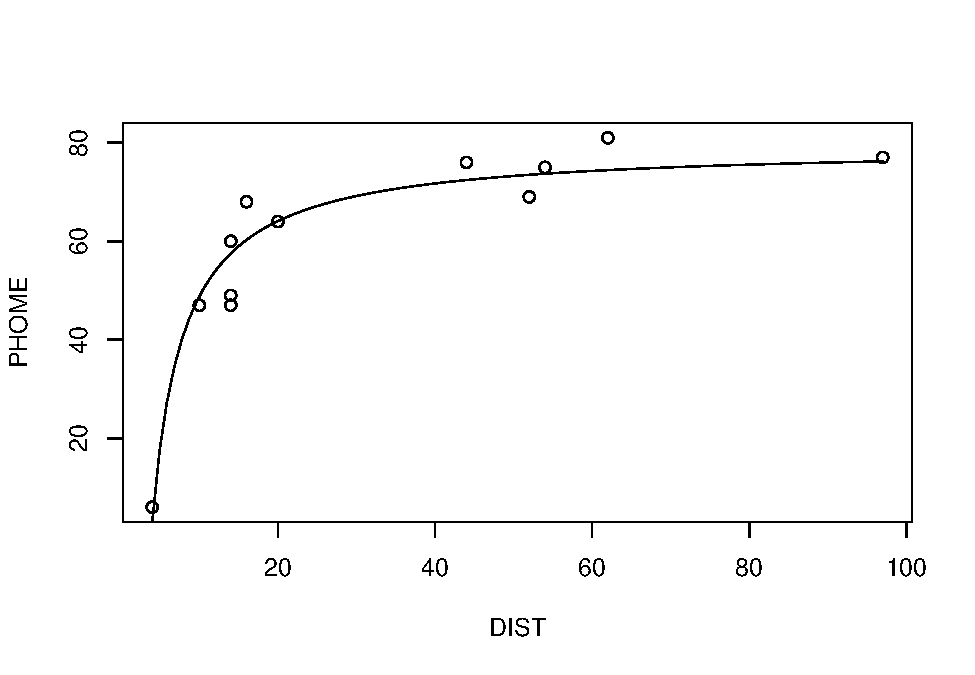
\includegraphics{Homework_7_files/figure-latex/unnamed-chunk-7-2.pdf}

与例7.8中斜率\(73.93\),截距\(-266.32\)相比,当去除\texttt{NANTUCKET}和\texttt{DUCKS}两个点后,获得的截距\(79\)更大,截距\(-305.52\)更小,由图可见,拟合得到的曲线更加贴合数据的走势。

仿照例7.8,绘制残差图

\begin{Shaded}
\begin{Highlighting}[]
\KeywordTok{plot}\NormalTok{(M2}\OperatorTok{$}\NormalTok{fitted.values,M2}\OperatorTok{$}\NormalTok{residuals,}\DataTypeTok{xlab =} \StringTok{'fitted'}\NormalTok{,}\DataTypeTok{ylab =} \StringTok{'residuals'}\NormalTok{)}
\KeywordTok{abline}\NormalTok{(}\DataTypeTok{h =} \DecValTok{0}\NormalTok{,}\DataTypeTok{lty =} \DecValTok{2}\NormalTok{)}
\end{Highlighting}
\end{Shaded}

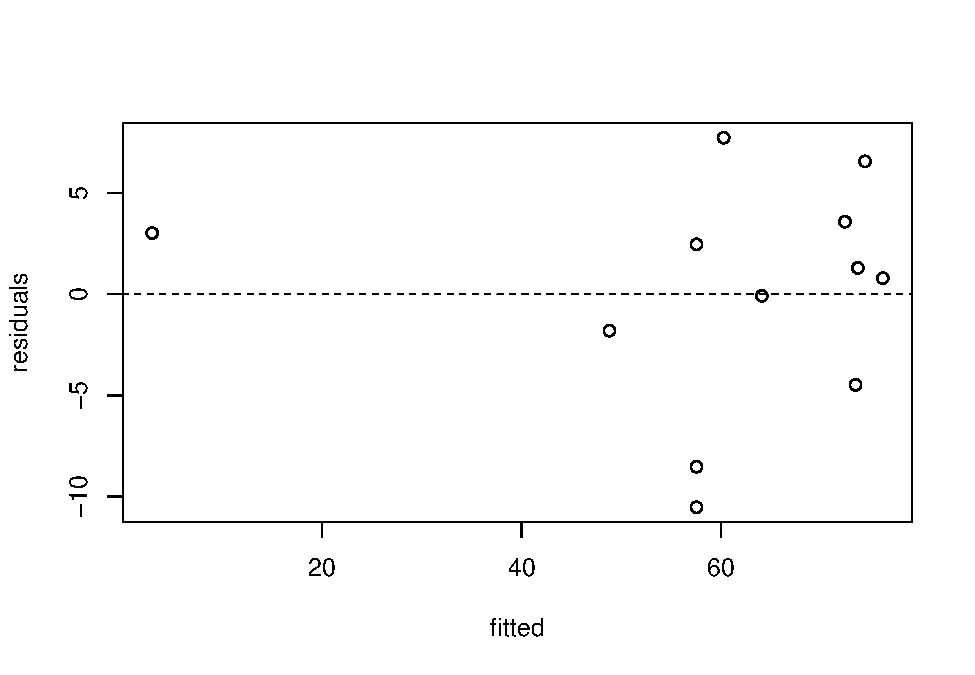
\includegraphics{Homework_7_files/figure-latex/unnamed-chunk-8-1.pdf}

相比例7.8,当去除\texttt{NANTUCKET}和\texttt{DUCKS}两个点后,残差范围更小,说明拟合效果更优。


\end{document}
